%% A brief test of different estimators of galaxy peculiar velocity
%% Sun Nov 29, 2015
%% Christopher Rooney

\documentclass[usenatbib]{mn2e}

%%%%%%%%%%%%%%%%%%%%%%%%%%%%%%%%%%%%%%%%%%%%%%%%%%%%%%%%%%%%%%%%%%%%%%
%% This section is called the preamble, where we can specify which
%% latex packages we required.  Most (but not of all) of the packages
%% below should be fairly standard in most latex documents.  The
%% exception is xspace and the new \latex command, which you probably
%% do not need.
%%%%%%%%%%%%%%%%%%%%%%%%%%%%%%%%%%%%%%%%%%%%%%%%%%%%%%%%%%%%%%%%%%%%%%

%% Bibliography style:
\usepackage{mathptmx}           % Use the Times font.
\usepackage{graphicx}           % Needed for including graphics.
\usepackage{url}                % Facility for activating URLs.
\usepackage{verbatim}           % For verbatiminput command.
\usepackage{booktabs}
%% Set the paper size to be letter, with a 2cm margin 
%% all around the page.
\usepackage{gensymb}

\newcommand{\iu}{{i\mkern1mu}}
\newcommand{\e}{{\mathrm e}}
\usepackage{xspace}
 

\voffset=-0.5truein
\textheight=9.5truein
\textwidth=6.5truein
\voffset=-0.55in
\hoffset=0.06in
\textwidth=6.4in
\textheight=9in
%
\def\gtwid{\mathrel{\raise.3ex\hbox{$>$\kern-.75em\lower1ex\hbox{$\sim$}}}}
\def\ltwid{\mathrel{\raise.3ex\hbox{$<$\kern-.75em\lower1ex\hbox{$\sim$}}}}
\def\lessim{\mathrel{\raise.3ex\hbox{$<$\kern-.75em\lower1ex\hbox{$\sim$}}}}
\def\\{\hfil\break}
\def\ie{{\it i.e.\ }}
\def\eg{{\it e.g.\ }}
\def\etal{{\it et al.\ }}
%\newcommand{\apj}{ApJ}

%Astro Stuff
%some units
\newcommand{\km}{\unit{km}}
\newcommand{\kms}{\unit{km~s\mone}}
\newcommand{\kpc}{\unit{kpc}}
\newcommand{\mpc}{\unit{Mpc}}
\newcommand{\hkpc}{\mamo{h\mone}\kpc}
\newcommand{\hmpc}{\mamo{h\mone}\mpc}
\newcommand{\parsec}{\unit{pc}}
\newcommand{\chisq}{\mamo{\chi^2}}
%
\newcommand{\hr}{\mamo{^{\rm h}}}
\newcommand{\m}{\mamo{^{\rm m}}}
%
\newcommand{\lb}[2]{\mamo{l = #1\arcdeg}, \mamo{b = #2\arcdeg}}
\newcommand{\dlb}[4]{\mamo{l = #1\fdg#2}, \mamo{b = #3\fdg#4}}
\newcommand{\lbapr}[2]{\mamo{l \approx #1\arcdeg}, \mamo{b \approx #2\arcdeg}}
%
\newcommand{\rightascen}{\mbox{R.A.}}
\newcommand{\declin}{\mbox{Dec.}}
\newcommand{\radec}[2]{\mamo{\alpha = #1^{\rm h}}, \mamo{\delta = #2\arcdeg}}
\newcommand{\dradec}[4]{\mamo{\alpha = #1\fh#2}, \mamo{\delta = #2\fdg#4}}
%
\newcommand{\xyz}[3]{($#1$, $#2$, $#3$)}
%
% useful abbreviations
\newcommand{\wrt}{with respect to}
\newcommand{\ebv}{\mbox{$E(B-V)$}}
\renewcommand{\lg}{\mamo{\sb{LG}}}
\newcommand{\cmb}{\mamo{\sb{CMB}}}
\newcommand{\rhat}{\mamo{\hat{\bfv{r}}}}
%
\newcommand{\secref}[1]{Section~\ref{sec:#1}}
\newcommand{\brref}[1]{(equation~\ref{eq:#1})}
%\newcommand{\eqref}[1]{equation~(\ref{eq:#1})}
\newcommand{\Eqref}[1]{Equation~(\ref{eq:#1})}
\newcommand{\figref}[1]{Fig.~\ref{fig:#1}}
\newcommand{\tabref}[1]{Table~\ref{tab:#1}}

\newcommand{\bt}{\mamo{B/T}}
\newcommand{\br}{\mamo{B-R}}
\newcommand{\del}{\mbox{d}}

\newcommand{\aap}{A\&A}
\newcommand{\apj}{ApJ}
\newcommand{\apjl}{ApJL}
\newcommand{\apjs}{ApJ Supp}
\newcommand{\aj}{AJ}
\newcommand{\mnras}{MNRAS}
\newcommand{\pasp}{PASP}
\newcommand{\prd}{Phys Rev D}
\begin{document}

\author{Christopher Rooney}
\date{\today}
\title{Distance Modulus Mistakes}
\maketitle

\begin{abstract}
In this document, I explore the differences between the astronomical ``Distance Modulus'' formula, and the approximation that I've been using, which is to just take the log of the distance. Special attention is given to the effects this has on the perturbation process.
\end{abstract}

\section{Introduction}
The usual distance modulus is as follows. Its physical meaning is that $\mu = m-M$ where $m$ is the apparent magnitude of the object and $M$ is it's absolute magnitude.
\begin{equation} \label{eq:modulus}
\mu_1 = 5\log\left(d\right) + 25
\end{equation}

The formula I've been using doesn't have a physical meaning, but has similar properties as the previous formula, especially the ``goes as the log of the distance'' part. It is as follows.

\begin{equation}\label{eq:log}
\mu_2 = \ln\left(d\right)
\end{equation}


\section{Theory}
First, a theoretical exploration was made of the two distance modulus formulas. A perturbation term was added to each equation. This term, $q$, can be thought of as a random number from a normal distribution with standard deviation 1 multiplied by the relative error number we're using (I've been using 0.1 for 10\% error).
\[
d_{p1} = e^{q_1\cdot\mu_1 + \mu_1}
\]

\[
d_{p2} = 10^{\left(q_2\cdot\mu_2 + \mu_2 - 25\right) / 5}
\]

I wanted to see how $q_1$ and $q_2$ were related, assuming that $d_{p1}=d_{p2}$. If they were proportional to each other, we would be able to find the constant of proportionality and simply change our relative error numbers to match. However, it was not that simple.

\[
\frac{q_1}{q_2} = 1 + \frac{5\cdot\ln\left(10\right)}{\ln\left(d\right)}
\]

Because this ratio depends on distance, it is impossible to fix the discrepancies simply by adjusting the constants we're putting into our fom



\section{Data}
I then tested everything numerically, resulting in Fig.~\ref{fig:distances}. A distance perturbed by 0.1 using Eq.~\ref{eq:log} is compared with the distance perturbed by 0.026 in Eq.~\ref{eq:modulus}. These values make the perturbed distances of the two methods equal at the arbitrary distance of 58 Mpc/h.
\begin{figure}
  \begin{center}
  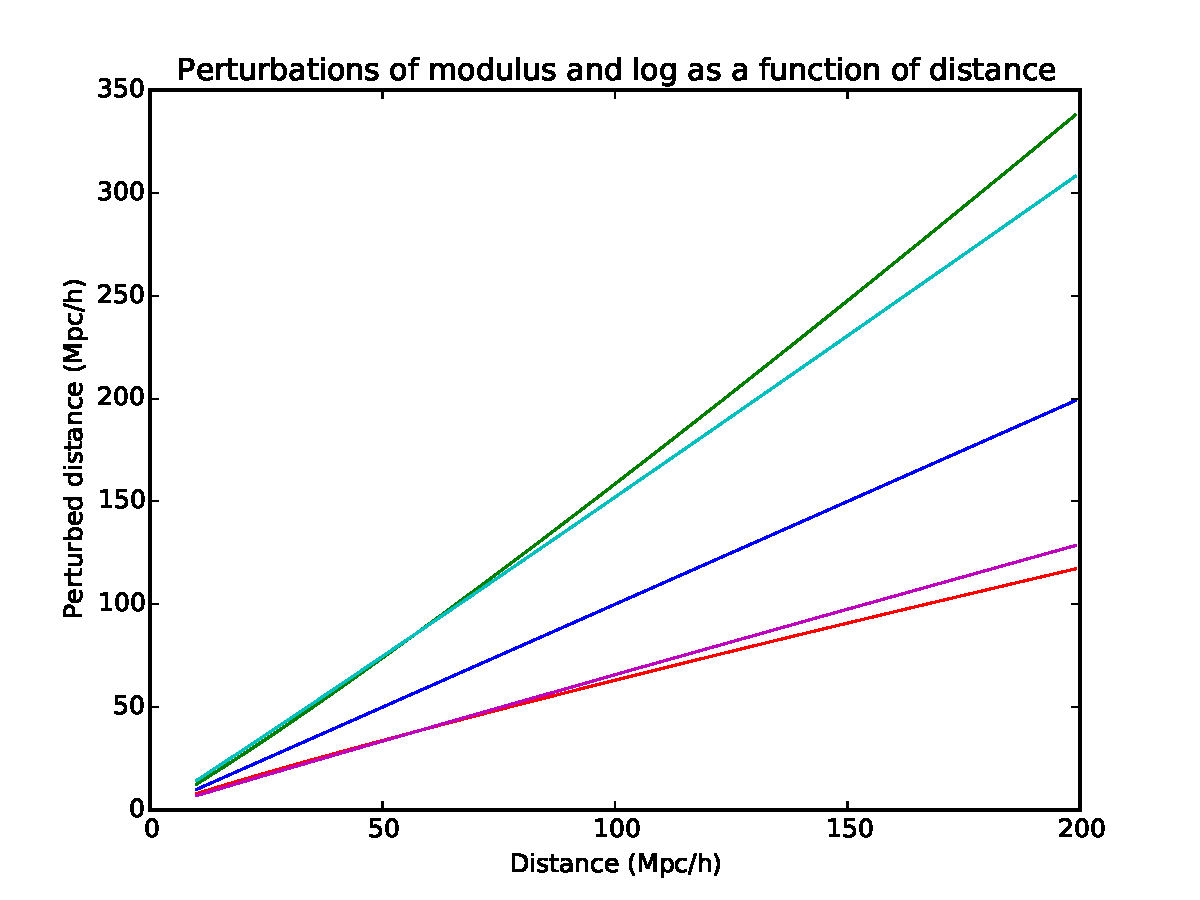
\includegraphics[scale=0.4]{moduluses.pdf}
  \end{center}
\caption{\small
Results of perturbing distances using the distance modulus formula and a straight natural log. Dark green and dark red (on the outside at large distances) are perturbed by $q_1 = \pm 0.1$. Cyan and magenta are the distances perturbed by $q_2 = \pm0.026$. Blue is the one-to-one line for comparison. 
}
\label{fig:distances}
\end{figure}

\section{Discussion and Conclusions}

Because I have proven that the two formulas are not equivalent, we will need to decide which to use in the end. One possible course would be to generate catalogs both ways and compare them. This could reveal artificial features produced by both approaches.

%%%%%%%%%%%%%%%%%%%%%%%%%%%%%%%%%%%%%%%%%%%%%%%%%%%%%%%%%%%%%%%%%%%%%%
%% Finally we specify the format required for our references and the
%% name of the bibtex file where our references should be taken from.
%%%%%%%%%%%%%%%%%%%%%%%%%%%%%%%%%%%%%%%%%%%%%%%%%%%%%%%%%%%%%%%%%%%%%%
\bibliographystyle{mn2e}
\bibliography{paper}
\end{document}

%%%%%%%%%%%%%%%%%%%%%%%%%%%%%%%%%%%%%%%%%%%%%%%%%%%%%%%%%%%%%%%%%%%%%%
%% The end.
%%%%%%%%%%%%%%%%%%%%%%%%%%%%%%%%%%%%%%%%%%%%%%%%%%%%%%%%%%%%%%%%%%%%%%
